\chapter{State of the Art}

  This chapter will review the classic methods used for localization and mapping, which is the core for any navigation technique, it starts describing the problems that arise both in localization and mapping. Continue with some of the most prolific solutions found to these problems to finish exposing the techniques and algorithms used by the Aerostack framework.

  Localization is referred to all the techniques used to find the position in coordinates of an agent or object inside the world, relative to a reference frame. As far as it's absolute coordinates are known, anything can be used as reference frame, it is used as the coordinates system's centre. In an outdoors environment, the Earth could be the reference frame and the robot's coordinates can be acquired with satellite systems, giving an absolute point inside the three dimensional space. It is desirable for these coordinates to be in a format that a computer can handle efficiently, tipically as two or three floating point numbers (although integer numbers are used sometimes too), depending on the number of dimensions used to represent the space. To save computational effort, the z axis (height) could be unused in a wheeled robot.

  Moving a robot avoiding possible obstacles through the space is tricky in itself, obstacles must be detected and handled correctly, moving objects can appear in the way, and so on. This alone does not provide any intelligence nor it helps planning, to aid in planning and moving smartly in the space, a map can be constructed while the localization is happening. The term mapping covers all the algorithms used to construct a map combining the data acquired from the many input sources a robot can have. Mapping opens the door for smart planning, along with many more advantages. A classic example is finding cycles in planned paths.

  \clearpage

  \section{Localization}

    Localization techniques are divided into two groups: Outdoor and indoor techniques. The distinction comes from the fact that satellite systems signals cannot go through walls. This fact has led to a whole new set of technologies and techniques that are able to localize in environments without an absolute reference of the world.

    This section is organized as follows: First outdoor localization will be analyzed, with a brief review of it's core components, then various indoor localization techniques will be exposed, focusing on lidar based techniques.

    \subsection{Outdoor localization} \label{ch_3:sect:localization:outdoor}

      By now, the most robust, reliable solution for outdoor localization is based on combining different sources of data. The mobile platform has drawn great attention over the past few years, pushing some of the largest companies in a shared effort to improve localization services while minimizing the impact over the battery's performance.

      Satellite systems localization in mobile applications have certain drawbacks: The most obvious one is that acquiring and processing the signal wastes power, but also that in the case of civilian systems (such as GPS) the localization has a precision of 10 meters for security reasons. Figure \ref{ch_3:fig:trilateration} shows the localization dissambiguation through the trilateration technique with three satellite.

      To aid both problems two new localization techniques were implemented:
      \begin{enumerate}
        \item GSM Localization. As every GSM antenna has a well known location stored in a database, one can localize trilaterating the near GSM antennas. Obviosly, this method is subject to GSM signal coverage.
        \item WiFi Localization. This powerful method can serve both as an indoor and outdoor localization technique (see sect. \ref{ch_3:sect:localization:indoor}). When a smarphone detects a WiFi hotspot, it sends it's BSSID along with the GPS coordinates if available to a centralized server. As this database grows the localization precision improves and every user can take advantage from it. This is scpecially useful in urban areas where stallite signal is poor or intermitent and improves as more and more users log information.
      \end{enumerate}

      The best localization services can be provided with the conjunction of these three main techniques, which can be easily merged with an \textit{Extended Kalman Filter}.

      \begin{figure}
        \centering
        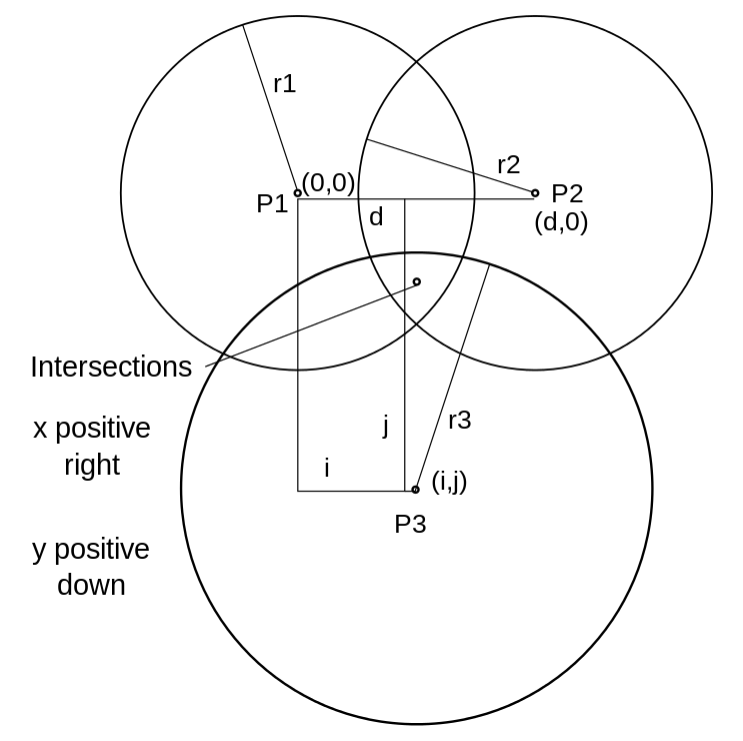
\includegraphics[width=0.6\textwidth]{./Figures/trilateration.png}
        \caption{The area enclosed by the three intersections ca be used to localize univocally. The three simple intersections formed by pairs of circumferences are always outside of the Earth. As more satellites are included, precision increases. Taken from \href{https://en.wikipedia.org/wiki/Trilateration}{wikipedia}}
        \label{ch_3:fig:trilateration}
      \end{figure}

      Although these techniques are widely used they are limited to mobile platforms, which are restricted both in sensorization and in processing capabilities. For robotic applications more sophisticated sensors are used, this includes depth cameras and lidars for the most part. Again, all the sensors output is merged to get the best estimates.

      In robotics, it is usual that the localization we are interested in is relative instead of absolute. This is done to aid in locating near objects in the space relative to the robot but also to construct a map, the process of localization and mapping simultaneously is called \textit{SLAM - Simultaneous Localization And Mapping} (see sect. \ref{ch_3:sect:localization:slam}).

    \subsection{Indoor localization} \label{ch_3:sect:localization:indoor}

      To localize in indoor environments many strategies can be followed, the general trend is to place different markers (active or passive) beforehand in well known locations. This markers are then recognized by the localizing device to know it's location. This \textit{recognizable markers} can be anything, a Bluetooth beacon, a WiFi hotspot, etc.

      Bluetooth beacons are specially crafted for this purpose as they can provide much more information. It has been extensively used in congresses and hotels to provide hosts with more information beyond localization, as services and timetables based on location. 

      In the case of WiFi hotspots localization is usually done by analyzing the signal strength and incoming angle. This method only works when the hotspots' location is known beforehand and is very prone to errors because the device must remain static in a certain angle.

      From the computer vision perspective, visual markers can be placed too and processed by the device localizing and again, this requires preparation beforehand. One example of this setup are the well known \href{https://www.uco.es/investiga/grupos/ava/node/26}{Aruco markers}.

      In many robotic applications like swarm robotics there is a necessity to track each member of the swarm in a closed, contained environment, for this purpose an \href{http://www.optitrack.com/}{OptiTrack} system can be used, it is a highly precise camera set that can track various markers (marked swarm members) and serve it's location through the network in real time. This setup is specially useful to monitor the swarm, enabling each member to access it's location.

    \subsection{SLAM} \label{ch_3:sect:localization:slam}

      SLAM is the process of mapping and, at the same time localizing inside that map. This is particularly useful in environments that are not prepared like the ones exposed previously, enabling the robot to work on an unknown place without getting lost nor entering cyclic paths. SLAM techniques are crucial in any robot with some degree of autonomy, it makes the navigation possible. 

      There are three main variants here, the ones based on Extended Kalman Filters, the probabilistic ones and the ones based on Graph Optimization.

    \subsubsection{Extended Kalman Filters SLAM} \label{ch_3:sect:localization:ekf}

      Extended Kalman Filters (EKF) SLAM is the earliest technique developed for SLAM. EKF is a general technique to find the best estimate for the measuring variable based on the mean and covariance. In this case the inputs are the odometry used to estimate the robot position, features of the environment that anchor the odometry measures and the robot motor system sensors (wheel decoders, etc) to estimate the change on the position. Then the objective is to find the best estimate for the current robot's position.

      \begin{figure}[!t]
        \centering
        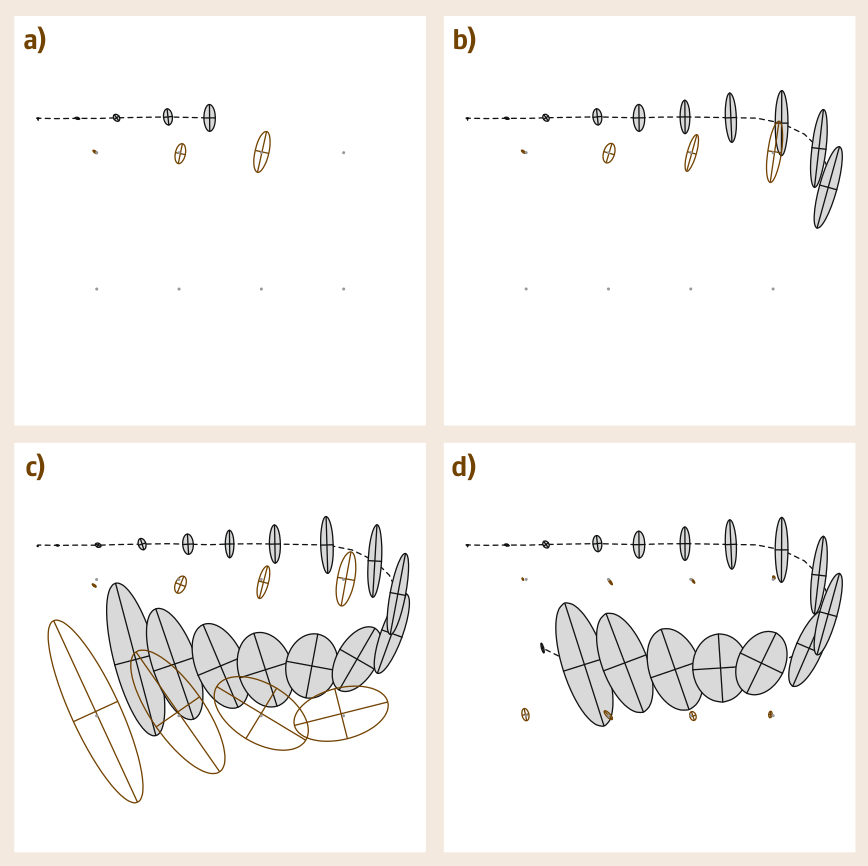
\includegraphics[width=0.8\textwidth]{./Figures/slam_ekf_model.png}
        \caption{EKF applied to the SLAM problem. Dotted line: robot's path. Shaded ellipses: position estimates. Small dots: Unkown location landmarks. White ellipses: Landmarks' position estimates. In (d) the robot senses the first landmark, anchoring the rest of the estimates, reducing uncertainty.}
        \label{ch_3:fig:ekf_slam}
      \end{figure}

      At the start of the process, the system's ($0$, $0$) coordinate is established where the robot is, this is the most confident measure about the robot position. As the robot navigates the environment, succesive measures are taken and paired with the known landmarks, when a previously seen landmark is witnessed again, the position estimate is corrected with the covariance matrix, and the error correction is propagated along the previous estimates. In this way a long as the robot is navigating an sensing the landmarks, the position estimate improves. Figure \ref{ch_3:fig:ekf_slam} shows the full process, in (a) the process is started, there is a lot of uncertainty, as process continues (a-c) the uncertainty increases, until the first landmark is sensed again (c), reducing the uncertainty on the current position's estimate and the subsequent estimates.

      More formally, the EKF algorithm represents the robot estimate by a multivariate Gaussian (\ref{ch_3:eq:ekf_representation})
      
      \begin{equation} \label{ch_3:eq:ekf_representation}
        p(x_{t}, m | Z_{t}, U_{t}) = N(\mu_{t}, \Sigma_{t})
      \end{equation}

      Where $\mu_{t}$ contains the robot's best estimate of its current location $x_{t}$ and the locations of all the landmarks, its size is $3 + 2N$, 3 points for the robot location and 2 for each of the $N$ landmarks. The matrix $\Sigma_{t}$ is the covariance of the expected error in the guess $\mu_{t}$ assessed by the robot, a square, dense matrix of $(3 + 2N) \times (3 + 2N)$.

      Although this technique works well on small maps, it renders unusable for large maps, this happens because the covariance matrix $\Sigma_{t}$ used to correlate the position estimates grows cuadratically with the measures, making the memory footprint wildly large and the overall processing time very high. Some researchers have proposed an improvement over the EKF SLAM algorithm through submap decomposition \cite{Guivant2001, Leonard2000}.

    \subsubsection{Particle Filters}

      Particle Filters are a probabilistic approach to position estimation, usually called Fast SLAM \cite{Montemerlo2002}. It uses various \textit{particles} that represent the posterior probability of the true distribution of maps and possible paths. To do so it stands over a method called Rao-Blackwellization, that aids in dimensioning the number of particles needed to represent the map. Also, as conditional indepence is assumed between the observed landmarks, every landmark can be represented as $N$ small Gaussians, which is linear, instead of exponential on the number of landmarks.

      At any point a set of $K$ particles is retained, where each particle has the form exposed in equation \ref{ch_3:eq:particle_form}.

      \begin{equation} \label{ch_3:eq:particle_form}
        X_{t}^{[k]}, \mu_{t,1}^{[k]}, \cdots, \mu_{t,N}^{[k]}, \Sigma_{t,1}^{[k]}, \cdots, \Sigma_{t,N}^{[k]}
      \end{equation}

      Where $k$ is the index of the path sample and $n$ the number of the landmark. This implies that every particle contains a sample path $X_{t}^{[k]}$ and a set of $N$ Gaussians $\approx (\mu_{t,n}^{[k]}, \Sigma_{t,n}^{[k]})$, one for each landmark.

      When a new odometry measure is received, it is combined with the previous knowledge through probabilistic sampling. A new location is generated for each particle, following a distribution based on the robot motion model and the previous measure of that particle ($x_{t-1}^{[k]}$). More specifically:

      \begin{equation} \label{ch_3:eq:particle_update}
        x_{t}^{[k]} \approach p(x_{t} | x_{t-1}^{[k]}, u_{t})
      \end{equation}

      Then, when a new measure $z_{t}$ is received, each particle's importance is weighted, assigning how important is that particle to that measure, this is the probability of that measure based on the particle's knowledge, defined in equaton \ref{ch_3:eq:particle_importance}. Let $n$ be the observed landmark's index:

      \begin{equation} \label{ch_3:eq:particle_importance}
        w_{t}^{[k]} = N(z_{t} | x_{t}^{[k]}, \mu_{t,n}^{[k]}, \Sigma_{t,n}^{[k]})
      \end{equation}

      After equation \ref{ch_3:eq:particle_importance} is applied for each particle, all the weights are normalized to sum up to 1, then a set new particles is drawn with replacement, where the probability of being picked is each particle weigth. Intuitively, this means that only the particles that fit the most with the current measures survive for next rounds. The final step of FastSLAM updates the mean $\mu_{t}^{[k]}$ and covariance $\Sigma_{t,n}^{[k]}$ based on the new measure $z_{t}$, which is similar to the EKF updates, but with much smaller filters.

      Although this method is easy to implement, fast enough for real time applications with not very high demanding software and yields good results on small to medium maps, it suffers from the fact that lots of particles are needed to represent big maps, specially with multiple nested loops. Therefore, many improvements have been proposed, \cite{Grisetti2007} for example uses ocucupancy grids instead of Gaussians.

    \subsubsection{Graph Optimization SLAM}

      The Graph Optimization SLAM techniques try to optimize a graphical model representing the landmarks and robot locations. In this representation, each location is viewed as a node in the graph, and the edge (called soft constraint) between two consecutive nodes is the captured odometry. The key intuition behind these methods is that at the end, the graph is sparse, because, each node will have just a few connections to other nodes. Also, at worst, the number of entries in the graph is linear in the time elapsed and in the number of nodes.

      This is the most widely used approach because sparse linear optimization is in a very advanced stage, allowing for scalable, yet efficient implementations of the algorithm.

    \subsubsection{Lidar SLAM}

      Lidar is a well established laser range sensor that can be used for depth estimation. By doing fast sweeps in 360 degrees it can compose a depth map which can be used for SLAM.

      Hector SLAM \cite{hector_slam} is a technique developed in the Darmstadt University. It uses a lidar sensor to do a fast SLAM by matching rays along sweeps.

      Along this work, the \textit{hector\_slam} ROS module will be integrated into the Aerostack framework, providing a robust SLAM technique ready to use for the drones equiped with lidar.

    \subsubsection{Visual SLAM}

      Using computer vision for SLAM have been a challange since it's conception, it raises the difficulty, specially for monocular cameras. Although many features can be extracted from images, it is not clear how to process nor store the data taking into account the full 6 degrees of freedom in a camera. All the parameters of the camera must be known beforehand, depth cameras include a lot of noise and monocular cameras do not have scale.

      In \cite{murTRO2015}, ORB-SLAM is proposed. Intuitively, it creates ORB features from a visual input and stores it in a sparse matrix, then a matching process is launched to localize every feature, improving the localization along the way. It can work on Monocular (no scale), Stereo and Depth Cameras, giving extraordinary results.

  This chapter reviewed the main adversities inherent to the SLAM problem and shed some light over the current state of the art. In the rest of this document, we will focus solely on lidar SLAM as the drones used with Aerostack are bound to lidar sensors. 

  \begin{comment}
    \begin{itemize}
    \end{itemize}
  \end{comment}
